\documentclass[emulatestandardclasses]{scrartcl}
\usepackage{graphicx}
\usepackage{color}
\usepackage[ngerman]{babel}
\usepackage{hyperref}
\usepackage{fullpage}
\usepackage{calc} 
\usepackage{enumitem}
\usepackage{titlesec}
\newcommand{\todo}[1]{\textcolor{red}{TODO: #1}\PackageWarning{TODO:}{#1!}}
\date{\vspace{-3ex}}
\begin{document}

\title{
	\includegraphics*[width=0.75\textwidth]{images/hu_logo.png}\\
	\vspace{24pt}
	Einf"uhrung in die Sprachphilosophie}
\subtitle{VEV WS 16/17\\
          Dr. Jasper Liptow\\
          Philosophisches Institut I \\ 
          Humboldt Universit"at zu Berlin}
\author{Lennard Wolf\\
        \small{\href{mailto:lennard.wolf@student.hu-berlin.de}{lennard.wolf@student.hu-berlin.de}}}
\maketitle
\begin{abstract}

Die Vorlesung soll grundlegendes Wissen "uber Probleme, Begriffe und Positionen der Sprachphilosophie des 20. Jahrhunderts vermitteln. Nach einer einf"uhrenden Einheit, in der das Ph"anomen der sprachlichen Bedeutung, das im Mittelpunkt sprachphilosophischer Untersuchungen steht, herausgearbeitet wird, widmen wir uns ausgew"ahlten systematischen Themen (wie etwa den verschiedenen Dimensionen sprachlicher Bedeutung, dem Zusammenhang von Bedeutung und Gebrauch sprachlicher Ausdr"ucke oder dem Verh"altnis von Sprache und Denken). Die Vorlesung wird von Tutorien begleitet, in denen Texte besprochen werden, die f"ur die Vorlesung eine Rolle spielen, und Fragen der Vorlesung vertieft diskutiert werden k"onnen.


\end{abstract}
\newpage

\tableofcontents
\newpage


\section{Einf"uhrungssitzung\\(24.10.16)}
\subsection{Organisatorisches}

\begin{itemize}
  \item Jede Woche begleitender Text der vorher zu lesen ist (bis 30.11. k"onnen runtergeladen werden)
  \item In Tutorien werden Texte nachbesprochen
  \item 4 Essays (3-4 Standardseiten) f"ur Tutorien zum Bestehen 
  \item Passwort: Platte
\end{itemize}

\subsection{Was ist Sprachphilosophie?}
\subsubsection{Die Methode der Sprachphilosophie}

Ziel der Sprachphilosophie ist es, Erkenntnisse "uber Sprache zu gewinnen, ohne Empirie anzuwenden. Dadurch sollen philosophische Fragen \emph{verschwinden}. Unterschiede zu Empirischer Forschung sind umstritten, und diese k"onnen in den folgenden zwei Weisen betrachtet werden.

\textbf{Unterschiede prinzipieller Natur:} Empirische Wissenschaft untersucht die Welt \emph{direkt}, Philosophie durch eine Analyse unserer Begriffe | Art der Rechtfertigung: \emph{a priori} vs. \emph{a posteriori} | Art der Belege: Erfahrung vs. Intuition | Modaler Status des Wissens: kontingente Wahrheiten (Empirie) vs. notwendige Wahrheiten (Philosophie).

\textbf{Unterschiede gradueller Natur:} `Abstraktheit': Philosophie untersucht besonders abstrakte oder allgemeine Aspekte ihres Gegenstands | `Semantischer Aufstieg': Philosophische Untersuchungen reflektieren in einem besonderen Ma\ss e über den Gehalt der Begriffe, mit denen sie operieren | Bezug zu `allt"aglichem Selbstverst"andnis': Philosophische Erkenntnisse bleiben an unser allt"agliches
Selbstverst"andnis zur"uckgebunden | Reflexion auf Zusammenh"ange: Philosophische Untersuchungen reflektieren in besonderer Weise darauf, wie ihre Gegenst"ande mit Gegenst"anden anderer Bereiche zusammenh"angen.


\subsubsection{Der Gegenstand der Sprachphilosophie}

Der zentrale Gegenstand der Sprachphilosophie ist das Ph"anomen der sprachlichen \emph{Bedeutung}. Es gibt vielf"altige \emph{Bedeutungen} einer Aussage im allt"aglichen Sinn, z.B. metaphorische \emph{Bedeutung}, ironische \emph{Bedeutung} und indirekte Mitteilung. Diese vielf"altigen \emph{Bedeutungen} lassen sich aber systematisch ordnen. Als \emph{erste Bedeutung} wird die buchst"abliche, oder auch w"ortliche Bedeutung bezeichnet.

\textbf{Grundfragen:} Was ist Bedeutung (im Sinn der \emph{ersten Bedeutung})? (Was hei\ss t es für einen sprachlichen Ausdruck, etwas zu bedeuten?) | Was heißt es für einen sprachlichen Ausdruck einer bestimmten Art, das zu bedeuten, was sprachliche Ausdr"ucke dieser Art bedeuten? | Wie h"angen die Bedeutungen verschiedener Arten von Ausdr"ucken zusammen? | Welches sind die (prim"aren) `Tr"ager' von Bedeutung? (W"orter? S"atze? "Au\ss erungen?) | Wie h"angt die \emph{erste Bedeutung} mit dem zusammen, was man durch die "Au\ss erung eines Satzes alles zum Ausdruck bringen kann? | Wie lassen sich die vielf"altigen Weisen unseres Gebrauchs von bedeutungsvollen S"atzen erkl"aren? | Wie h"angt sprachliche Bedeutung mit anderen Ph"anomenen (Absichten, Konventionen) zusammen?

\newpage



\section{Frege: "Uber Sinn und Bedeutung I\\(31.10.16)}

\subsection{Vornotizen zum Text}
\subsubsection{Inhalt des Textes}
\begin{itemize}
  \item \emph{R"atsel}: Wie kann $a = b$ einen anderen Erkenntniswert als $ a = a$ haben wenn es wahr ist? $\rightarrow$ \emph{Sinn} 
  \item \emph{Antwort}: Liegt nicht an dem unterschiedlichen Bezug (Bedeutung$_{F}$) und auch nicht an den unterschiedlichen Ausdr"ucken
  \item Zeichen (Eigenname) $\rightarrow$ Sinn (das \emph{Gemeinte}) $\rightarrow$ Bedeutung$_{F}$ (\emph{Auf das gedeutet wird})
  \item \textbf{Beispiel} -- \emph{Zeichen}: Abendstern $\rightarrow$ \emph{Sinn}: ein bestimmtes Himmelsgestirn $\rightarrow$ \emph{Bedeutung}: Venus 
  \item Bei dem Zeichen \emph{Morgenstern} w"are die Bedeutung$_{F}$ identisch, aber der Sinn w"are m"oglicherweise ein anderer
  \item Der Sinn eines Eigennamens ist die \emph{Art des Gegebensein}.
  \item Der Sinn eines Satzes ist der \emph{Gedanke} (objektiver Inhalt der nicht ein Prozess in einem Kopf ist sondern von vielen gedacht werden kann) den er ausdr"uckt.
  \item Die Bedeutung$_{F}$ eines Satzes ist sein Wahrheitswert.
  \item \emph{Das Streben nach Wahrheit also ist es, as uns "uberall vom Sinn zur Bedeutung$_{F}$ vorzudringen treibt.}
  \item Das \emph{Urteil} ist der Fortschritt von einem Gedanken zu seinem Wahrheitswert
\end{itemize}
\subsubsection{Fragen}
\begin{itemize}
  \item Ist Bedeutung nur in realer Welt (kontextunabh"angig) oder kann in zB einem literarischen Kontext eine Bedeutung vorhanden sein? (kontextsensitiv, Stichwort Odysseus)
\end{itemize}

\subsection{The Linguistic Turn}

Man kann das 20. Jahrhundert als Jahrhundert der Sprachphilosophie bezeichnen, denn Sprache war zentraler Gegenstand philosophischer Untersuchung. So wie es in verschiedenen Jahrhunderten  immer K"onigsdisziplinen gab (z.B. Ontologie, Epistemologie etc.), so also auch zu der Zeit. Sprachphilosophische Untersuchungen spielen eine Rolle in beinahe allen Bereichen der Philosophie, und sprachphilosophische Untersuchungen sollten so die Frage nach dem Wesen der Philosophie selbst kl"aren. War Sprachphilosophie also eine neue `Erste Philosophie'?

Bis dahin wurden in der Philosophie Untersuchungen von Sprache nur gelegentlich und unsystematisch, und vor allem nur im Rahmen von Logik, Rhetorik und Sprachkritik durchgef"uhrt. Dies kommt daher, dass bis Ende des 19. Jahrhunderts Sprache (bis auf einzelne Ausnahmen) lediglich als Ausdruck eines im Wesentlichen \emph{sprachunabh"angigen Denkens} begriffen wird. Philosophisch interessant war nur die Beziehung zwischen \emph{Denken} (Geist, Seele) und Welt. Doch Gedanken wie dass Denken wesentlich von Sprache abh"angig ist verhalfen zum \emph{Linguistic Turn}.


\subsection{Die Grundfrage der Sprachphilosophie}

Im Zentrum der Sprachphilosophie befindet sich das Problem sprachlicher Bedeutung: Wie ist es zu verstehen, dass sprachliche "Au\ss erungen und die Ausdr"ucke, mit denen sie vollzogen werden, etwas bedeuten? Wie ist es zu verstehen, dass wir einander durch sprachliche "Au\ss erungen etwas über die Welt zu verstehen geben k"onnen? (Sprachliche Bedeutung meint hier zun"achst die \emph{erste Bedeutung} einer "Au\ss erung oder eines Ausdrucks.

\subsection{Naive Bedeutungstheorien}

Als `Naive Bedeutungstheorien' k"onnen Bedeutung als Vorstellungen sowie Bedeutung als objektive Gegenst"ande genannt werden. Wenn man diese genauer betrachtet, fallen einige Probleme auf. Bei der Theorie der Bedeutung als Vorstellungen k"ame u.a. das Problem des Weltbezugs auf (Wenn die Bedeutungen von W"ortern damit verbundene Vorstellungen sind, dann handeln unsere "Au\ss erungen nicht von der Welt selbst, sondern von unseren Vorstellungen von der Welt). Bei der Theorie der Bedeutung als objektive Gegenst"ande st"o\ss t man auf \emph{Freges R"atsel}. \\


\textbf{Wichtig:}\\Seite 42, Fu\ss note 2\\
Lesen: \emph{Der Gedanke }von Frege


\section{Frege: "Uber Sinn und Bedeutung II\\(07.11.16)}


\textbf{Bis Frege:} Theorie der Bedeutung sprachlicher Ausdr"ucke als Theorie der Bedeutung von Namen\\
\textbf{Nach Frege:} Theorie der Bedeutung sprachlicher Ausdr"ucke als Theorie des Aufbaus under Abh"angigkeit der Bedeutung der verschiedenen Arten sprachlicher Ausdr"ucke einer Sprache (\emph{Bedeutungstheorie})


\begin{description}[leftmargin=!,labelwidth=\widthof{\bfseries 2}]
  \item[Eigenname$_{F}$] Ausdr"ucke, die die Funktion haben, f"ur einen einzelnen Gegenstand zu stehen (vgl. 41). Dies umfasst \emph{echte Eigennamen} wie `Sokrates', \emph{Pronomen} wie `dies' oder `der', \emph{definite Kennzeichnungen} wie `der Schnittpunkt der Geraden $a$ und $b$' | Heute spricht man von \emph{singul"aren Termen}, wobei keine Einigkeit dar"uber besteht, ob `definite Kennzeichnungen' tats"achlich singul"are Terme sind.
  \item[Bedeutung$_{F}$ eines Eigennamen$_{F}$] Das Bezeichnete | ein bestimmter Gegenstand
  \item[Sinn$_{F}$ eines Eigennamen$_{F}$] Das, worin die Art des Gegebenseins enthalten ist | die Art, in der der Ausdruck seine Bedeutung$_{F}$ pr"asentiert oder herausgreift.
  \item[Beziehung Sinn$_{F}$ - Bedeutung$_{F}$] Keine Bedeutung$_{F}$ ohne Sinn$_{F}$; Jedoch Sinn$_{F}$ geht ohne Bedeutung$_{F}$ | Zwei Eigennamen$_{F}$ mit selbem Sinn$_{F}$, m"ussen dieselbe Bedeutung$_{F}$ haben | Zwei Eigennamen$_{F}$ k"onnen dieselbe Bedeutung$_{F}$ haben, aber unterschiedlichen Sinn$_{F}$.
  \item[Sinn$_{F}$ eines Satzes] Der \emph{Gedanke}, der von einem Satz zum Ausdruck gebracht wird | Anders als bei Eigennamen$_{F}$: Wir k"onnen den Sinn$_{F}$ von S"atzen nicht erlernen | Das Erfassen der Gedanken, die von S"atzen zum Ausdruck gebracht werden, h"angt mit dem Erfassen des Sinns$_{F}$ der Ausdr"ucke zusammen, aus denen die S"atze aufgebaut sind.
  \item[Bedeutung$_{F}$ eines Satzes] Der \emph{Wahrheitswert},  des Satzes, d.h. der `Umstand, da\ss~er wahr oder da\ss~er falsch ist'.
  \item[Gedanke] Kein psychischer Akt, sondern ein objektiver Inhalt, der gemeinsames Eigentum von vielen sein kann | Heute spricht man von \emph{Propositionen (im Fregeschen Sinn)}. 
  \item[Kompositionalit"at des Sinns$_{F}$] Wenn ich in einem Satz einen Ausdruck mit einem anderen, welcher den selben Sinn$_{F}$ hat, dann "andert sich der Sinn$_{F}$ des Satzes nicht. {\color{red}???}
  \item[Kompositionalit"at der Bedeutung$_{F}$] Wenn ich in einem Satz einen Ausdruck mit einem anderen, welcher die selbe Bedeutung$_{F}$ hat, dann "andert sich die Bedeutung$_{F}$ des Satzes nicht.
  \item[Satz] Seit Frege: Satz ist vollst"ndig, wenn er einen \emph{Gedanken} zum Ausdruck bringt, einen \emph{Wahrheitswert} hat und wir mit ihm \emph{sprachliche Handlungen} vollziehen k"onnen.
  \item[Kontextprinzip] Sprachliche Ausdr"ucke unterhalb der Satzebene (`W"orter') haben (in einem strikten Sinn) nur im Kontext vollst"andiger S"atze Bedeutung
    \item[Pr"adikat] Sprachebene: Pr"adikate; Weltebene: Eigenschaften | Wahrheitsfunktion
\end{description}

\textbf{Freges Entscheidender Gedanke} Der logisch einfache Satz ist nicht aus zwei (oder mehr) gleichartigen Elementen zusammengef"ugt, sondern zerf"allt in Ausdr"ucke, die sich in ihrer sprachlichen Funktion wesentlich voneinander unterscheiden. (Singul"are Terme [Frege: \emph{Eigenname}], die auf etwas Bezug nehmen und Pr"adikate [Frege: \emph{Begriffsw"orter}], die auf die Gegenst"ande zutreffen m"ussen) | Quine: Pr"adikate sind offene S"atze (`\emph{$x$ ist ein kl"uger als $y$}')

\section{Russell: "Uber das Kennzeichnen\\(21.11.16)}

\subsection{R"uckblick: Semantische Grundgedanken im Anschluss an Frege}

\begin{itemize}
  \item Ein Satz ist keine blo\ss e Aneinanderreihung von Namen: singul"are Terme werden in Leerstellen der Pr"adikate eingesetzt
  \item () ist weise. $\rightarrow$ (Sokrates) ist weise.
  \item Primat des Satzes: Verst"ndnis dessen, was die Bedeutung eines sprachlichen Ausdrucks ausmacht setzt ein Verst"ndnis dessen voraus was ein Satz und seine Bedeutung ausmacht.
  \item Der Sinn des Satzes ist der Gedanke, den der Satz ausdr"uckt.
  \item Dieser Sinn ergibt sich vollst"andig aus der Form des Satzes und die Sinne seiner Ausdr"ucke.
  \item Wir k"onnen den Sinn eines Satzes verstehen ohne zu wissen ob er wahr oder falsch ist.
  \item Der Sinn eines Satzes bestimmt was der Fall sein muss damit er wahr ist.
  \item Wir verstehen einen Satz \emph{nur} dann, wenn wir wissen, was der Fall ist, wenn er wahr ist. (\emph{notwendig})
\end{itemize}

\subsection{Einw"ande Russels zu Frege}
\begin{itemize}
  \item Frege verkennt die logische Funktion von \emph{definiten Kennzeichnung}.
  \item Frege verkennt den Charakter sprachlicher Bedeutung von echten singul"aren Termen (Dimension des Sinns ist "uberfl"ussig, Referenz ist f"ur Bedeutung konstitutiv)
  \item Frege verkennt was es "uberhaupt f"ur einen Ausdruck hei"st, etwas zu bedeuten (nicht fu"r alle Ausdr"ucke l"asst sich Sinn und Bedeutung angeben)
\end{itemize}

\subsection{Gr"unde f"ur die Relevanz von Russels Theorie}
\begin{itemize}
  \item Er zeigt wie eine Untersuchung der Sprache philosophische Probleme betreffen k"onnte.
  \item Er zeigt wie die logisch-semantische Form von S"atzen von ihrer grammatischen Form abweichen k"onnte.
  \item Er zeigt eine (gute) Alternative zu einer Fregeianischen Konzeption von Bedeutung auf.
\end{itemize}

\subsection{Begriffe}

\begin{description}[leftmargin=!,labelwidth=\widthof{\bfseries Gebrauchsdefinition}]
    \item[Kennzeichnung] Ein Ausdruck, der grammatisch die Rolle eines singul"aren Terms spielt... | Ausdruck ist Kennzeichnung \emph{genau dann wenn} er grammatisch die Rolle eines singul"aren Terms spielt [\emph{denoting phrase}]
    \item[Pr"adikat] Beispiel: (...) \emph{ist klug}. $\rightarrow C(...)$
    \item[Aussage] Pr"adikat in dessen Leerstelle eine Variable eingesetzt wurde ($x$ \emph{ist klug}.) | Beispiele: $C($Nichts$)$ bedeutet $\forall x~\neg C(x)$ | $C($Alles$)$ bedeutet $\forall x~C(x)$ | $C($Etwas$)$ bedeutet $\neg \forall x~\neg C(x)$ | [\emph{proposition}]
    \item[Gebrauchsdefinition] Kennzeichnung haben f"ur sich nie eine Bedeutung. Daher k"onnen sie nur im Kontext von S"atzen definiert werden| \emph{Nicht:} `Alles bedeutet...', sondern `S"atze der Form \emph{F"ur alles gilt C.} bedeuten...'  
    \item[Definite Kennz.]Haben niht Funktion auf einzelnen Gegenstand Bezug zu nehmen. Sie sind keine ingul"aren Terme. | Bedeutung definiter Kennzeichungen l"asst sich nur dadurch angeben, dass man die Bedeutung vollst"andiger S"atze angibt, in denen sie vorkommen.\\`Der/die/das F ist C' bedeutet $\exists x~(F(x) \wedge C(x) \wedge \forall y~(F(y) \rightarrow y = x) )$
    \item[Extension] 
    \item[Intension] 
\end{description}

\subsection{Probleme}

\begin{description}[leftmargin=!,labelwidth=\widthof{\bfseries Probl. des Bezugs}]
    \item[Probl. des Bezugs] unerf"ullter Kennzeichnungen. | Zu Meinong: Wenn wir denken, dass Dinge existieren m"ussen, damit die S"atze in denen sie vorkommen nicht unsinnig sind, machen wir `schr"age' metaphysische Annahmen. | Zu Frege: `Der K"onig von Frankreich hat eine Glatze.' ist nicht unsinnig, sondern falsch! | Russels Theorie l"ost das Problem durch die Erkenntnis, dass Kennzeichnungen Existenz implizieren.
    \item[Freges R"atsel] Frage nach Erkenntniswert von Identit"atsaussagen wie $a = b$ im Gegensatz zu $a = a$. Russels Theorie l"ost das Problem dadurch, dass nach ihm Identit"atsaussagen die nur \emph{a posteriori} als wahr eingesehen werden k"onnen nicht die Form $a = b$ haben, sondern (explizit oder implizit) mindestens eine definite Kennzeichung enthalten. | Problem: Was ist mit Eigennamen? (`Hesperus ist identisch mit Phosphorus.') $\rightarrow$ Russell: Eigennamen \emph{bedeuten} ihre Kennzeichnung.
    \item[...] ................
\end{description}

\subsection{Russell vs. Frege}

...


\section{Krippke: Name und Notwendigkeit I\\(14.11.16)}

\subsection{Lekt"ure}

\noindent\textbf{Hintergund}

Kripke kritisiert an Freges und Russells Ideen, dass dort Eigennamen als Abk"urzungen zu Kennzeichnungen verstanden werden. Er stellt in Frage, dass Aristoteles synonym mit `der ber"uhmteste Sch"uler von Platon' ist. Vielmehr k"onnten sie Abk"urzungen f"ur Kennzeichnungsb"undel sein, doch auch dies stellt sich als kurzsichtig und zu vereinfachend heraus. Schlussendlich m"ochte er keine Theorie vorstellen sondern nur klarer zeigen, dass die bisherigen Ansichten nicht ausreichen.\\

\subsection{R"uckblick}

\textbf{Bisheriges Bild der Sprache}
Sprache ist Medium einer besonderen Form der \emph{Kommunikation} | Kern der sprachlichen Kommunikation:"Au"sern und Verstehen der buchst"ablichen ersten Bedeutung von S"atzen | S"atze besitzen Wahrheitsbedingungen |Kompositionalit"atsprinzip: Grammatik erlaubt Konstruktion unendlich vieler S"atze. Jedoch: bisher Beschr"ankung auf Aussages"atze; was ist mit Frage-, Befehls-, Handlungss"atzen; andere Aspekte der Kommunikation?

\begin{description}[leftmargin=!,labelwidth=\widthof{\bfseries Definite Kennzeichnung}]
    \item[Ausdruckarten] Junktoren; Quantoren
    \item[a priori] 
    \item[a posteriori] 
    \item[kontingent] 
    \item[notwendig]
    \item[Name] Namen sind starre Bezeichnungsausdr"ucke (\emph{rigid designators}). Es ist nicht m"oglich, dass der Name `Aristoteles', so wie wir ihn gebrauchen, einen anderen Gegenstand bezeichnet als den, den er tats"achlich bezeichnet.
    \item[Definite Kennzeichnung] Definite Kennzeichnung sind nicht so starr. ...?
\end{description} 

\section{Krippke: Name und Notwendigkeit II\\(28.11.16)}

\subsection{Deskritivistische Auffassungen von Namen}  

Jeder Name hat eine \emph{Bedeutung}. Die Referenz von Namen auf Gegenst"ande kann auf das Zutreffen von Kennzeichnungen auf Gegenst"ande zuruckgef"uhrt werden.

F"ur jeden Namen `$X$', den eine Sprecherin $S$ verwendet, soll gelten:

\begin{description}[leftmargin=!,labelwidth=\widthof{\bfseries (B)}]
    \item[(1)] Jedem Namen oder Bezeichnungsausdruck `$X$' entspricht ein B"undel von Eigenschaften, n"amlich die Familie der Eigenschaften $\varphi$, f"ur die gilt: $A$ meint `$\varphi X$'.
    \item[(2)] $A$ meint, dass eine der Eigenschaften oder einige Eigenschaften zusammen einen bestimmten individuellen Gegenstand als einzigen herausgreifen.
    \item[(3)] Wenn die meisten oder eine ausschlaggebende Menge der $\varphi$'s von einem einzigen Gegenstand $y$ erf"ullt werden, dann ist $y$ der Referent von `$X$'.
    \item[(4)] Wenn die Abstimmung nicht einen einzigen Gegenstand liefert, dann referiert `$X$' nicht.
    \item[(5)] Die Aussage "`Wenn $X$ existiert, dann hat $X$ die meisten der $\varphi$'s"' wei"s der Sprecher \emph{a priori}.
    \item[(6)] Die Aussage "`Wenn $X$ existiert, dann hat $X$ die meisten der $\varphi$'s"' dr"uckt eine notwendige Wahrheit aus (im Idiolekt des Sprechers).
    \item[(B)] F"ur jede gelungene Theorie gilt, dass die Erkl"arung nicht zirkul"ar sein darf. Die Eigenschaften, welche bei der Abstimmung verwendet werden, d"urfen nicht selbst den Begriff der Referenz auf eine Weise enthalten, die seine Eliminierung letztlich unm"oglich macht.
\end{description}

\subsection{Kripkes Kirtik des Deskriptivismus}

\begin{description}[leftmargin=!,labelwidth=\widthof{\bfseries (1)}]
    \item[(6) ist falsch] Es ist nicht notwendig, dass Aristoteles die meisten der Eigenschaften besitzt, die ihm gew"ohnlich zugeschrieben werden.
    \item[(5) ist falsch] Das gew"ohnliche Wissen von SPrecherinnen dar"uber, welche Eigenschaften die Referenten ihrer Namen besitzen, ist \emph{a posteriori}.
    \item[(3) ist falsch] Selbst wenn nicht Aristoteles, sondern jemand anders die meisten Eigenschaften h"atte, die wir gew"ohnlich Aristoteles zuschreiben, w"urde `Aristoteles' auf Aristoteles referieren.
    \item[(2) ist falsch] Viele, die den Namen `Feynman' verwenden und damit auf Feynman referieren, wissen nicht mehr "uber Feynman als dass dieser ein ber"uhmter Physiker war.
\end{description}

\subsection{Kripkes kausale `Theorie' der Namen}

Die Referenz eines Namens beinhaltet in den grundlegenden F"allen) das Bestehen einer `Kommunikationskette'. Hierbei handelt es sich um eine \emph{kausale} Beziehung zwischen dem Referenten und der SPrecherin, die darin besteht, dass (1.) dem Referenten der Name in einer ursppr"unglichen Taufe \emph{demonstrativ} oder durch eine Kennzeichnung gegeben wird, und dass (2.) ....??

Das Bestehen einer Kommunikationskette ist vielleicht eine \emph{notwendige}, aber keine \emph{hinreichende} Bedingung. Zum Beispiel kann die Sprecherin beabsichtigen, einen anderen Gegenstand zu referieren, als es die H"orer es verstehen.\\

\noindent \textbf{Probleme}\\
Wie lassen sich fiktionale Gegenst"ande (falls es sie gibt) `taufen'? Kann es sein dass `Aussagen "uber nicht existierende Gegenst"ande' eigentlich sinnlos sind?\\
Namen scheinen ihre Referenz ver"andern zu k"onnen. (vgl. Evans: \emph{The Causal Theory of Names}) $\rightarrow$ Die `urspr"ungliche Taufe' scheint problematisch.

\subsection{`Nat"urliche Art Ausdr"ucke' (\emph{Natural Kind Terms})}

Ausdr"ucke f"ur Substanzen oder Arten von Gegenst"anden, wie sie in unserer nat"urlichen Umwelt vorkommen und von den Naturwissenschaften kategorisiert werden (`Wasser', `Gold', `Zitone').\\
Deskritivistische Auffassungen von Namen l"asst sich hier "ahnlich gut anwenden: Die `Taufe' w"are \emph{demonstrativ} (`"Wass ist alles, das von derselben nat"urlichen Art ist, wie \emph{das} hier.'"). $\rightarrow$ `derselben nat"urlichen Art' = Sie haben \emph{dasselbe Wesen}\\
Nat"urliche Art Ausdr"ucke sind entsprechend auch \emph{rigid designators}. .... \textbf{copy paste here pls}

\subsection{Internalismus vs. Externalismus}

\begin{description}[leftmargin=!,labelwidth=\widthof{\bfseries Semantischer Externalismus}]
    \item[Semantischer Internalismus] ...
    \item[Semantischer Externalismus] ...
    \item[Kausaler Externalismus] ...
    \item[Sozialer Externalismus] ...
\end{description}

Externalismus ist einer der wichtigesten philosophischen Gedanken des 20. Jh., weg von der kartesianischen Auffassung der Sprache. 



\section{Grice I\\(05.12.16)}

\subsection{Intensionalistische Bedeutungstheorien}


\begin{itemize}
  \item Geist ist das Fundament der Sprache: Deswegen Intentionalit"at (Searle)
  \item Traditionell: Sprachliche Ausdr"ucke stehe f"ur Ideen (Locke) $\rightarrow$ keine psychologischen Konzeptionen der Bedeutung
\end{itemize}

\begin{description}[leftmargin=!,labelwidth=\widthof{\bfseries Semantischer Externalismus}]
    \item[Intentionalit"at] Gerichtetheit (Brentano) 
\end{description}

\subsubsection{Das "`Grice'sche Programm"'}

\begin{description}[leftmargin=!,labelwidth=\widthof{\bfseries 11}]
    \item[1] Die konventionelle Bedeutung sprachlicher Ausdr"ucke wird zur"uckgef"uhrt auf die Bedeutung der der "Au"serungen einzelner Sprecherinnen.
    \item[2] Die Bedeutung der "Au"serungen einzelner Sprecherinnen wird zur"uckgef"uhrt auf die Gehalte der geistigen Zust"ande einzelner Sprecherinnen.
    \item[3] Die Gehalte der geistigen Zust"ande einzelner Sprecherinnen werden zur"uckgef"uhrt auf die (nichtsprachliche) kausale Interaktion dieser Zust"ande mit der Welt (und miteinander).
\end{description}

\subsubsection{Grice' Methode}

\begin{description}[leftmargin=!,labelwidth=\widthof{\bfseries 11}]
    \item[1] "`Analyse"' des Bedeutungsbegriffs
    \item[2] Angabe dessen, was "Au"serungen fer Form "`$x$ bedeutet etwas"' oder "`$x$ bedeutet dass $p$"' bedeuten
\end{description}

\noindent \textbf{Mindestanforderung an eine gelungene Analyse eines Begriffs $F$:}\\
Formulierung eines \emph{wahren} Bikonditionals der Form "`$x$ ist $F$ genau dann, wenn $x$ .... ist"' ($F$ darf rechts nicht sein, wie auch keine von $F$ abh"angigen Begriffe)

\subsection{Grice' Analyse des Meinens}


\begin{description}[leftmargin=!,labelwidth=\widthof{\bfseries 11}]
    \item[Analyse 1] (falsch)
    \item[Analyse 2] (falsch)
\end{description}

\noindent \textbf{Erl"auterungen}

\begin{description}[leftmargin=!,labelwidth=\widthof{\bfseries 11}]
    \item[Absicht] Nicht blo"s "`explizite"' Pl"ane oder "`vorg"angige"' Absichten, sondern auch "`implizite"' Absichten oder \emph{intentions in action} (Searle)
    \item[Erkenntnis der Absicht] ...
\end{description}

\noindent \textbf{Bemerkungen}
Es geht nur um \emph{Aussages"atze} | Imperative:


\subsection{Tutorium}

\begin{itemize}
  \item Es geht nun um die Bedeutungstheorie, im besonderen um Absichten, durch die Bedeutung entsteht
  \item Sprecher Bedeutung erkl"art Wort/Satz-Bedeutung
  \item Nat"urlich: Flecken bedeuten Masern. (Notwendige Bedeutung)
  \item Nicht-nat"urlich: Klingeln bedeutet, dass der Bus voll ist.
\end{itemize}

\noindent $S$ meint$_{NN}$ mit $x$, dass $p$ gdw. $S$ die Absicht hat, 

\begin{description}[leftmargin=!,labelwidth=\widthof{\bfseries 3}]
    \item[1] beim H"orer die "Uberzeugung dass $p$ hervorzurufen
    \item[2] dass der H"orer die Absicht (1) erkennt
    \item[3] dass die Absicht (1) erf"ullt wird, weil der H"orer (2) erkennt.
\end{description}


\section{Grice II\\(12.12.16)}

\subsection{Das Programm in seiner "`Reinform"'}

Gebrauchstheorie der Bedeutung als Gegensatz zu Intentionaler Gebrauchstheorie\\
Inspiriert von Wittgensteins \emph{Philosophischen Untersuchungen}

\begin{itemize}
  \item Sprachliche Bedeutung kann vollst"ndig in Begrifen ihres Gebrauchs erkl"art werden, ohne dabei auf mentale Zust"ande und Ereignisse Bezug zu nehmen.
  \item Der Gehalt mentaler Zust"ande und Ereignisse kann auf die Bedeutung sprachlicher Ausdr"ucke zur"uckgef"uhrt werden. (mentale Ereignisse als "`innere Rede"', mentale Zust"ande als Dispositionen zu sprachlichen "Au"serungen)
\end{itemize}

\subsection{Gebrauchstheorien der Bedeutung}

\begin{description}[leftmargin=!,labelwidth=\widthof{\bfseries Erl"auterung}]
    \item[Grundidee] Bedeutung eines Ausdrucks wird durch in einer Sprachgemeinschaft geltenden Regeln seines Gebrauchs konstituiert ("`Gebrauch"' als eine Form des regelm"a"sigen oder regelgeleiteten Verhaltens)
    \item[Erl"auterung] Analogie mit Spiel: Sprache als ein Spiel mit Ausdr"ucken als "`Spielsteinen"' und "Au"serungen als "`Z"ugen"'. (Vgl. Wittgensteins Begriff des Sprachspiels, PU, \S 6)
    \item[Folgerungen]Sprachen sind soziale, regelgeleitete Praktiken des Gebrauchs sprachlicher Ausdr"ucke | Die Bedeutung eines Ausdrucks ist nichts anderes als die Gesamtheit der \emph{Regeln seines Gebruachs}. | Das "`Subjekt"' eines Sprache ist in erster Linie nicht eine einzelne Sprecherin, sondern ein \emph{Kollektiv}, eine Sprecher\emph{gemeinschft}. | Was ein Ausdruck bedeutet ist unabh"angig davon, was \emph{einzelne Sprecherinnen} mit der "Au"serungen.....??? | Sprache ist ein wesentlich soziales Ph"anomen.
\end{description}

\subsection{Antisystematische Gebrauchstheorien}


\subsection{Systematische Gebrauchstheorien}

Wittgenstein: Bringt nichts!

\subsection{Tutorium}

\emph{Language has a downtown} -- Es gibt einen Sprachkern auf dem Improvisationsm"oglichkeiten aufbauen


\section{Davidson: Wahrheit und Bedeutung\\(09.01.17)}

\subsection{Die Systematizit"at sprachlicher Bedeutung}

\begin{description}[leftmargin=!,labelwidth=\widthof{\bfseries Ausgangspunkt}]
    \item[Ausgangspunkt] Wir m"ussen erkl"aren, wie Bedeutung der S"atze von Bedeutung der W"orter abh"angt, weil sonst die Lernbarkeit nicht erkl"art werden kann (unendlichkeit der Sprache ist von endlichen Wesen erlernbar) | Ziel: Erkl"arung der Kompositionalit"at (wurde vorher noch nicht getan), nicht die der Bedeutung einzelner Worte!
    \item[Modell] Annette bezieht sich auf Annette, der Vater von bezieht sich auf eine Person die das erf"ullt $\rightarrow$ Bezugspunkt wird \emph{abgeleitet}
    \item[Konsequenzen] Ausdr"ucke m"ussen nicht immer eine zugeordnete Entit"at sein, sondern kann sich darin ersch"opfen, "`eine systematische Wirkung zu haben in denen er vorkommt"' | Die F"ahgkeit, bedeutungsvolle S"atze zu verstehen, kann mit einer endlichen, empirischen Theorie (Bedeutungstheorie f"ur eine bestimmte Sprache) erkl"art werden. (Modell unserer Sprachverstehenskompetenz)
\end{description}

\subsection{Bedeutungstheorie f"ur eine nat"urliche Sprache}

\begin{description}[leftmargin=!,labelwidth=\widthof{\bfseries Herausforderungen}]
    \item[Herausforderungen] Sinn muss angegeben werden, nicht nur der \emph{Bezug} | f"ur jeden m"oglichen Satz muss explizit gezeigt werden k"onnen, wie die Bedeutung verstanden wird
    \item[Bedeutung] \emph{nicht} hilfreich: Wie k"onnen wir ableiten, dass "`Hans sitzt"' bedeutet \emph{Hans sitzt}?
    \item[Tarski] Davidsons Vorschlag: Tarskis "`semantische Definition der Wahrheit"' als Bedeutungstheorie benutzen (Tarski: \emph{Der Wahrheitsbegriff in den formalisierten Sprachen}, 1935) | Informationen "uber die Bedeutung von Ausdr"ucken: "`sitzt"' trifft auf jeden Gegenstand zu der sitzt. $\rightarrow$ "`Hans sitzt"' ist genau dann wahr wenn \emph{Hans sitzt}. aber: ist das eine Bedeutungsangabe?
    \item[Behauptung] Wenn man die Wahrheitsbedingungen f"ur einen Satz kennt, dann versteht man die Bedeutung dieses Satzes auch! 
\end{description}

Das ist eine theoretische Herausforderung, kein Argument.

\section{Austin: Performative "Ausserungen\\(16.01.17)}

\subsection{Bisher}

\begin{description}[leftmargin=!,labelwidth=\widthof{\bfseries Ausgangspunkt}]
    \item[Sprachlicher Ausdruck] Konstative/Assertorische S"atze ("`Das ist rot."'), haben Wahrheitswert
    \item[Fehlschluss] Alle "Au"serungen sind Behauptungen
\end{description}

\subsection{Sprachliche Bedeutung und sprachliches Handeln}

\begin{description}[leftmargin=!,labelwidth=\widthof{\bfseries Performative "Au"serungen}]
    \item[Sprechakttheorie] Anerkennung der Pluralit"at von Arten sprachlicher Handlungen (Behauptungen, Versprechen, Fragen, Bitten, Befehle etc.) | Versuch der systematischen Klassifikation und einer Erkl"arung der Unterschiede und Zusammenh"ange der verschiedenen Arten sprachlichen Handelns 
    \item[Performative "Au"serungen] "Au"serungen, die \emph{nicht} die Funktion haben, eine Behauptung zu machen. ("`Ich schw"ore."', "`Ich bitte um Verzeihung."', "`Ja ich will dich heiraten."') | K"onnen \emph{misslingen} im Gegensatz zu \emph{wahr/falsch sein} bei Behauptungen
    \item[Performativit"at] 
\end{description}

\subsection{Bedeutung und Kraft von "Ausserungen}

\begin{description}[leftmargin=!,labelwidth=\widthof{\bfseries Perlokution"arer Akt}]
    \item[Lokution"arer Akt] Bezeichnung der Eigenschaft eines Teilakts des Sprechaktes, und zwar des Teilaktes, der aus der sprachlichen "Au"serung (Phonetik, Grammatik, Semantik) besteht | Das "Au"sern eines Satzes mit einer bestimmten \emph{Bedeutung} (der Akt des Etwas Sagens)
    \item[Illokution"arer Akt] zielgerichtet; auf ein kommunikatives Ziel ausgerichtet; die Absichten des Sprechers zum Ausdruck bringend | Das "Au"sern eines Satzes mit einer bestimmten \emph{Kraft} | paradigmatische Form des \emph{Berichts} von Akten ($S~\phi$t, dass $p$)
    \item[Perlokution"arer Akt] Bezeichnung f"ur einen Teilakt des Sprechaktes, und zwar für die Wirkung, die die sprachliche "Au"serung (Phonetik, Grammatik, Semantik) auf den H"orer hat. | Das Hervorbringen bestimmter Wirkungen in der Zuh"orerschaft durch das "Au"sern eines Satzes mit einer bestimmten Kraft
\end{description}

\subsection{Arten des Misslingens}

\begin{description}[leftmargin=!,labelwidth=\widthof{\bfseries Perlokution"arer Akt}]
    \item[Keine Konvention] 
    \item[Ungeeignete Verh"altnisse] Zu einem Pferd: "`Ich ernenne Sie zum Pr"asidenten."'
    \item[Keine Intention] Jemand hat zum Beispiel vorher nicht die n"otigen Rechte bekommen.
    \item[Unter Zwang] 
\end{description}

Dass es sich dabei um Sprachakte handelt ist aber kontingent.

\section{Searle: Performative "Ausserungen\\(23.01.17)}

\subsection{Illokution"are Akte}

\begin{description}[leftmargin=!,labelwidth=\widthof{\bfseries Illokution"arer Akt}]
    \item[Illokution"arer Akt] Als \emph{kleinste Einheit sprachlicher Verst"andigung} $\rightarrow$ 
    \item[These] Der Vollzug illokution"arer Akte wird durch entsprechende \emph{Regeln} konstituiert. 
    \item[Idee] Eine Theorie illokution"arer Akte hat die Form einer \emph{Explikation} dieser Regeln. 
\end{description}

\subsection{Regeln}

\begin{description}[leftmargin=!,labelwidth=\widthof{\bfseries Konstitutive Regel}]
    \item[Regulative Regel] Logisch unabh"angig von der geregelten T"atigkeit | Regelausdruck in Form des Imperativs: "`Wenn $Y$, tue $X$"'
    \item[Konstitutive Regel] Logisch abh"angig von der geregelten T"atigkeit | Regelausdruck in Form einer Definition:  "`$X$ gilt als $Y$"'
\end{description}

\section{Grice: Logik und Konversation\\(30.01.17)}


\section{Davidson: Vern"unftige Tiere\\(06.02.17)}

\subsection{Sprache und Denken: m"ogliche Thesen}

\begin{description}[leftmargin=!,labelwidth=\widthof{\bfseries These der partiellen Bedingtheit}]
    \item[Zur"uckf"uhrbarkeits-Thesen] Sprechen als externalisiertes Denken (Locke) / Denken als internalisiertes Sprechen (Dewey)
    \item[Bedingtheits-Thesen] Sprache als notwendige Bedingung des Denkens / Denken als notwendige Bedingung der Sprache
    \item[These der partiellen Bedingtheit] Sprache als notwendige Bedingung f"ur bestimmte \emph{Bereiche} des Denkens
    \item[Determiniertheits-These]
\end{description}

\subsection{Die Intensionalist"at von Gedankenberichten}

\begin{description}[leftmargin=!,labelwidth=\widthof{\bfseries \emph{de dicto}-Lesart}]
\item[\emph{de dicto}-Lesart] "`Hans glaubt, dass der Morgenstern ein Planet ist."' $\rightarrow$ Hans glaubt etwas, das sich so sagen l"asst: Der Morgenstern ist ein Planet.
\item[\emph{de re}-Lesart] "`Hans glaubt, dass der Morgenstern ein Planet ist."' $\rightarrow$ Hans glaubt \emph{von dem Morgenstern} etwas, das sich so sagen l"asst: \emph{er} ist ein Planet.
\end{description}

\subsection{Tutorium}


\begin{itemize}
  \item 
\end{itemize}


\newpage
%\section{"Uber den Dozenten}
%Dr. Jasper Liptow absolvierte 1996 seinen Magister an der Universit"at Hamburg, promovierte in Gie\ss en mit einer Arbeit zum Thema \emph{Gebrauchstheorien der Bedeutung} bei Prof. Martin Seel und ist Privatdozent.
%
%
%\begin{figure}[]
%	\centering
%	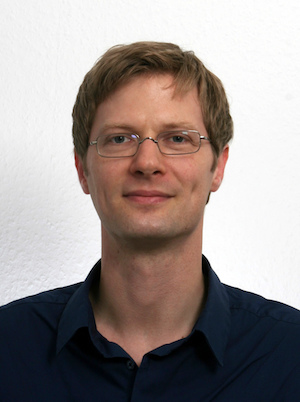
\includegraphics[width=0.32\textwidth]{images/liptow.jpg}
%	\caption{Dr. Jasper Liptow. Quelle: \url{https://www.uni-frankfurt.de/45457854/liptow.jpg}}
%	\label{fig:liptow}
%\end{figure}

%\begin{figure}[h]
%	\centering
%	
\includegraphics[width=0.5\textwidth]{images/template.png}
%	\caption{Template Bild}
%	\label{fig:template}
%\end{figure}

\end{document}
